\begin{frame}{Scientific Method}
	\textbf{Science is not a linear process.}

	The common Scientific method is an
	oversimplification.

	\begin{figure}
		\centering
		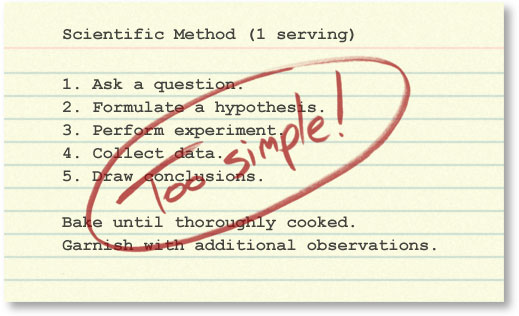
\includegraphics[width=0.7\textwidth]{Figures/sciencerecipe.jpg}
		\caption{The myth of the step-by-step science recipe. \cite{Science}}
	\end{figure}

\end{frame}

\begin{frame}{Then... How Does Science Actually Work?}
	\begin{columns}

		\column{0.6\textwidth}
		\textbf{Science revolves around four interconnected cores:}

		\vspace{0.3cm}
		\begin{itemize}
			\item \textbf{Observation} – Gathering data from the world.
			\item \textbf{Testing} – Evaluating Hypotheses.
			\item \textbf{Feedback} – Refining and adjusting ideas with the Community.
			\item \textbf{Applications} – Using scientific knowledge for Society.
		\end{itemize}

		\column{0.4\textwidth}
		\begin{figure}
			\centering
			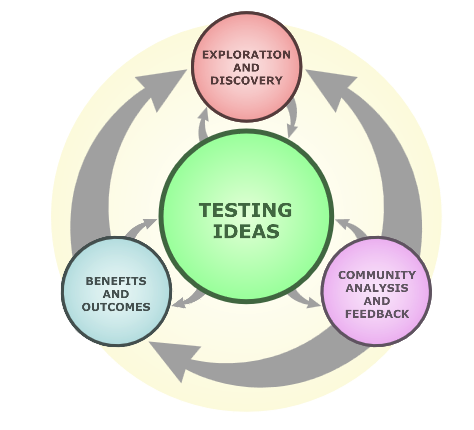
\includegraphics[width=\textwidth]{Figures/canvas.png}
			\caption{Interconnected nature of scientific processes. \cite{Science}}
		\end{figure}

	\end{columns}
\end{frame}

\begin{frame}{The Main Core: Testing Ideas}
	The heart of science is \textbf{testing ideas.}

	Through experimentation and analysis, hypotheses are refined, rejected, or strengthened.
	\begin{figure}
		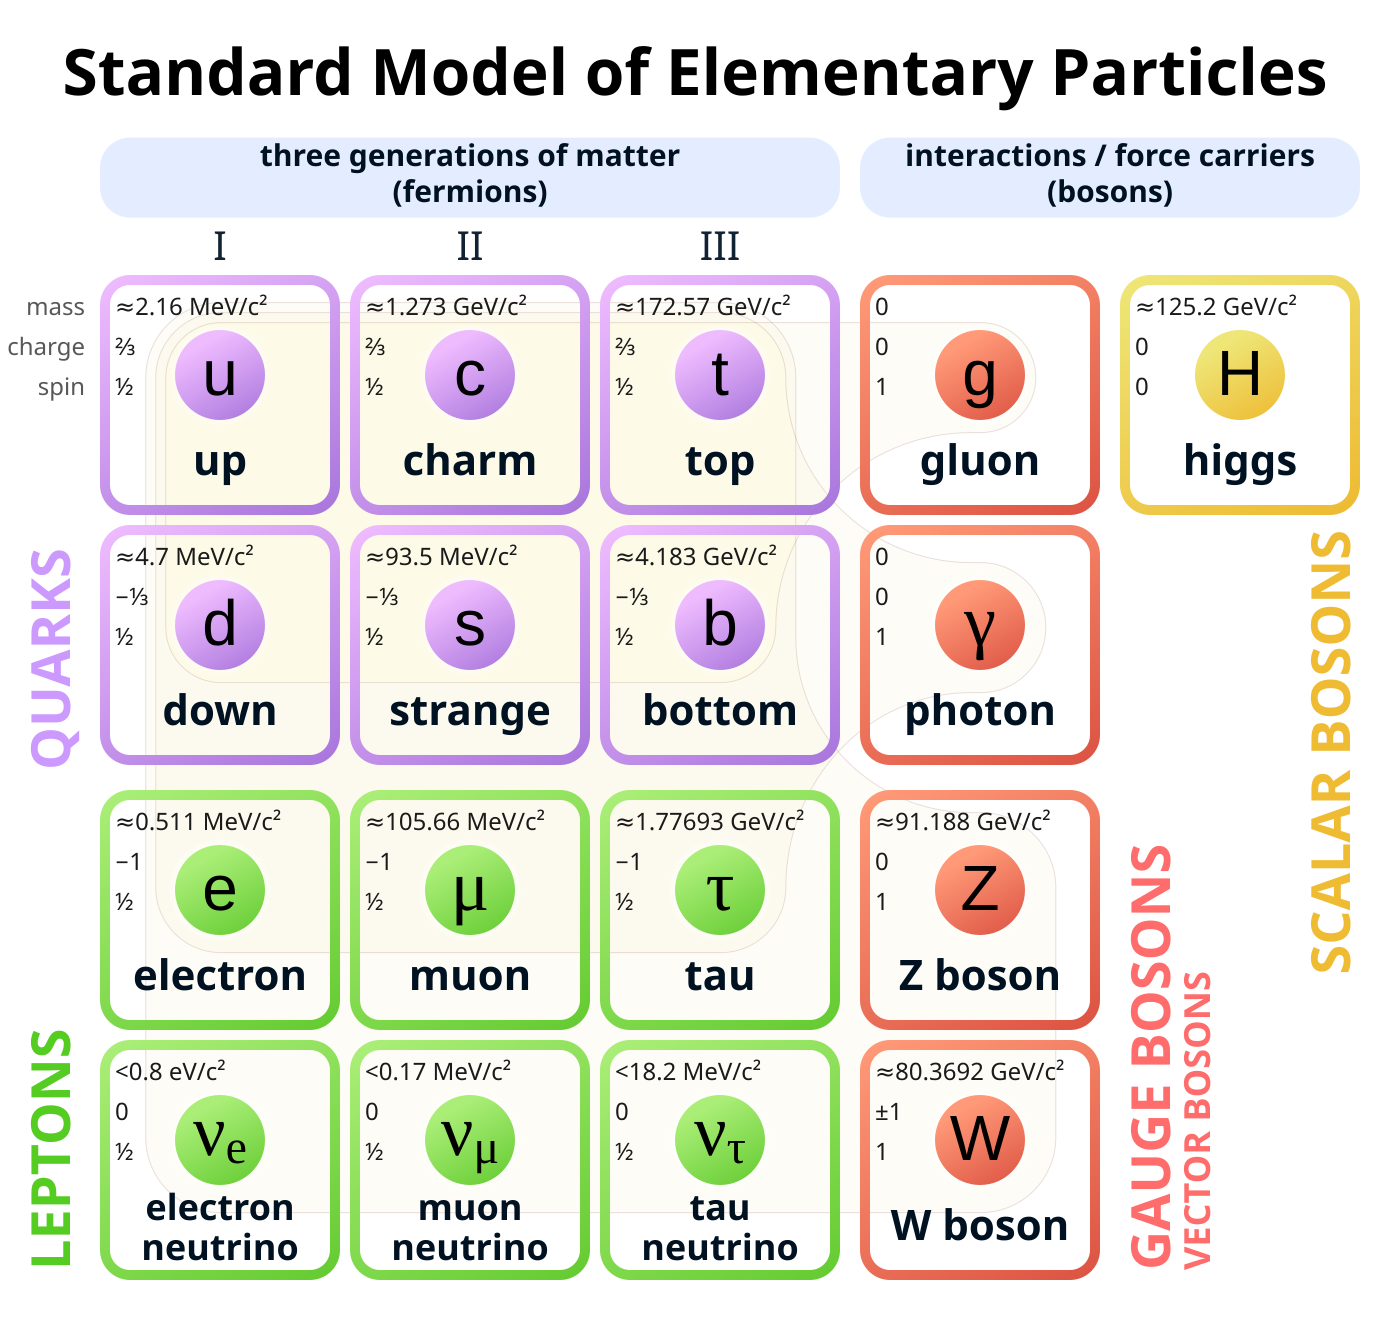
\includegraphics[width=0.5\textwidth]{Figures/Standard-Model.png}
		\caption{Elementary Particles of the Standard Model. \cite{Cush2019}}
	\end{figure}

\end{frame}
